\documentclass[10pt]{article}
\usepackage{tikz}
\usetikzlibrary{shapes.misc}
\usepackage[margin=0cm]{geometry}
\pagestyle{empty}
\tikzstyle{every node}=[cross out, draw, red]

\begin{document}

\vspace*{\fill}
\begin{center}
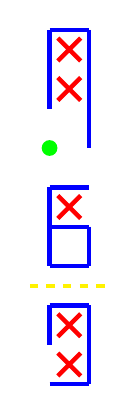
\begin{tikzpicture}[x=0.5cm, y=-0.5cm, ultra thick, blue]
% Walls
    \draw (0,0) -- (1,0);
    \draw (0,4) -- (1,4);
    \draw (0,5) -- (1,5);
    \draw (0,6) -- (1,6);
    \draw (0,7) -- (1,7);
    \draw (0,9) -- (1,9);
    \draw (0,0) -- (0,2);
    \draw (0,4) -- (0,6);
    \draw (0,7) -- (0,8);
    \draw (1,0) -- (1,3);
    \draw (1,5) -- (1,6);
    \draw (1,7) -- (1,9);
% Pillars
    \fill[green] (0,3) circle(0.2);
% Inner points in accessible cul-de-sacs
    \node at (0.5,0.5) {};
    \node at (0.5,1.5) {};
    \node at (0.5,4.5) {};
    \node at (0.5,7.5) {};
    \node at (0.5,8.5) {};
% Entry-exit paths without intersections
    \draw[dashed, yellow] (-0.5,6.5) -- (1.5,6.5);
\end{tikzpicture}
\end{center}
\vspace*{\fill}

\end{document}
